\documentclass[]{article}
\usepackage{lmodern}
\usepackage{amssymb,amsmath}
\usepackage{ifxetex,ifluatex}
\usepackage{fixltx2e} % provides \textsubscript
\ifnum 0\ifxetex 1\fi\ifluatex 1\fi=0 % if pdftex
  \usepackage[T1]{fontenc}
  \usepackage[utf8]{inputenc}
\else % if luatex or xelatex
  \ifxetex
    \usepackage{mathspec}
  \else
    \usepackage{fontspec}
  \fi
  \defaultfontfeatures{Ligatures=TeX,Scale=MatchLowercase}
\fi
% use upquote if available, for straight quotes in verbatim environments
\IfFileExists{upquote.sty}{\usepackage{upquote}}{}
% use microtype if available
\IfFileExists{microtype.sty}{%
\usepackage{microtype}
\UseMicrotypeSet[protrusion]{basicmath} % disable protrusion for tt fonts
}{}
\usepackage[margin=1in]{geometry}
\usepackage{hyperref}
\hypersetup{unicode=true,
            pdftitle={analysis},
            pdfauthor={Joshua Rosenberg},
            pdfborder={0 0 0},
            breaklinks=true}
\urlstyle{same}  % don't use monospace font for urls
\usepackage{color}
\usepackage{fancyvrb}
\newcommand{\VerbBar}{|}
\newcommand{\VERB}{\Verb[commandchars=\\\{\}]}
\DefineVerbatimEnvironment{Highlighting}{Verbatim}{commandchars=\\\{\}}
% Add ',fontsize=\small' for more characters per line
\usepackage{framed}
\definecolor{shadecolor}{RGB}{248,248,248}
\newenvironment{Shaded}{\begin{snugshade}}{\end{snugshade}}
\newcommand{\KeywordTok}[1]{\textcolor[rgb]{0.13,0.29,0.53}{\textbf{#1}}}
\newcommand{\DataTypeTok}[1]{\textcolor[rgb]{0.13,0.29,0.53}{#1}}
\newcommand{\DecValTok}[1]{\textcolor[rgb]{0.00,0.00,0.81}{#1}}
\newcommand{\BaseNTok}[1]{\textcolor[rgb]{0.00,0.00,0.81}{#1}}
\newcommand{\FloatTok}[1]{\textcolor[rgb]{0.00,0.00,0.81}{#1}}
\newcommand{\ConstantTok}[1]{\textcolor[rgb]{0.00,0.00,0.00}{#1}}
\newcommand{\CharTok}[1]{\textcolor[rgb]{0.31,0.60,0.02}{#1}}
\newcommand{\SpecialCharTok}[1]{\textcolor[rgb]{0.00,0.00,0.00}{#1}}
\newcommand{\StringTok}[1]{\textcolor[rgb]{0.31,0.60,0.02}{#1}}
\newcommand{\VerbatimStringTok}[1]{\textcolor[rgb]{0.31,0.60,0.02}{#1}}
\newcommand{\SpecialStringTok}[1]{\textcolor[rgb]{0.31,0.60,0.02}{#1}}
\newcommand{\ImportTok}[1]{#1}
\newcommand{\CommentTok}[1]{\textcolor[rgb]{0.56,0.35,0.01}{\textit{#1}}}
\newcommand{\DocumentationTok}[1]{\textcolor[rgb]{0.56,0.35,0.01}{\textbf{\textit{#1}}}}
\newcommand{\AnnotationTok}[1]{\textcolor[rgb]{0.56,0.35,0.01}{\textbf{\textit{#1}}}}
\newcommand{\CommentVarTok}[1]{\textcolor[rgb]{0.56,0.35,0.01}{\textbf{\textit{#1}}}}
\newcommand{\OtherTok}[1]{\textcolor[rgb]{0.56,0.35,0.01}{#1}}
\newcommand{\FunctionTok}[1]{\textcolor[rgb]{0.00,0.00,0.00}{#1}}
\newcommand{\VariableTok}[1]{\textcolor[rgb]{0.00,0.00,0.00}{#1}}
\newcommand{\ControlFlowTok}[1]{\textcolor[rgb]{0.13,0.29,0.53}{\textbf{#1}}}
\newcommand{\OperatorTok}[1]{\textcolor[rgb]{0.81,0.36,0.00}{\textbf{#1}}}
\newcommand{\BuiltInTok}[1]{#1}
\newcommand{\ExtensionTok}[1]{#1}
\newcommand{\PreprocessorTok}[1]{\textcolor[rgb]{0.56,0.35,0.01}{\textit{#1}}}
\newcommand{\AttributeTok}[1]{\textcolor[rgb]{0.77,0.63,0.00}{#1}}
\newcommand{\RegionMarkerTok}[1]{#1}
\newcommand{\InformationTok}[1]{\textcolor[rgb]{0.56,0.35,0.01}{\textbf{\textit{#1}}}}
\newcommand{\WarningTok}[1]{\textcolor[rgb]{0.56,0.35,0.01}{\textbf{\textit{#1}}}}
\newcommand{\AlertTok}[1]{\textcolor[rgb]{0.94,0.16,0.16}{#1}}
\newcommand{\ErrorTok}[1]{\textcolor[rgb]{0.64,0.00,0.00}{\textbf{#1}}}
\newcommand{\NormalTok}[1]{#1}
\usepackage{graphicx,grffile}
\makeatletter
\def\maxwidth{\ifdim\Gin@nat@width>\linewidth\linewidth\else\Gin@nat@width\fi}
\def\maxheight{\ifdim\Gin@nat@height>\textheight\textheight\else\Gin@nat@height\fi}
\makeatother
% Scale images if necessary, so that they will not overflow the page
% margins by default, and it is still possible to overwrite the defaults
% using explicit options in \includegraphics[width, height, ...]{}
\setkeys{Gin}{width=\maxwidth,height=\maxheight,keepaspectratio}
\IfFileExists{parskip.sty}{%
\usepackage{parskip}
}{% else
\setlength{\parindent}{0pt}
\setlength{\parskip}{6pt plus 2pt minus 1pt}
}
\setlength{\emergencystretch}{3em}  % prevent overfull lines
\providecommand{\tightlist}{%
  \setlength{\itemsep}{0pt}\setlength{\parskip}{0pt}}
\setcounter{secnumdepth}{0}
% Redefines (sub)paragraphs to behave more like sections
\ifx\paragraph\undefined\else
\let\oldparagraph\paragraph
\renewcommand{\paragraph}[1]{\oldparagraph{#1}\mbox{}}
\fi
\ifx\subparagraph\undefined\else
\let\oldsubparagraph\subparagraph
\renewcommand{\subparagraph}[1]{\oldsubparagraph{#1}\mbox{}}
\fi

%%% Use protect on footnotes to avoid problems with footnotes in titles
\let\rmarkdownfootnote\footnote%
\def\footnote{\protect\rmarkdownfootnote}

%%% Change title format to be more compact
\usepackage{titling}

% Create subtitle command for use in maketitle
\newcommand{\subtitle}[1]{
  \posttitle{
    \begin{center}\large#1\end{center}
    }
}

\setlength{\droptitle}{-2em}

  \title{analysis}
    \pretitle{\vspace{\droptitle}\centering\huge}
  \posttitle{\par}
    \author{Joshua Rosenberg}
    \preauthor{\centering\large\emph}
  \postauthor{\par}
      \predate{\centering\large\emph}
  \postdate{\par}
    \date{9/13/2018}


\begin{document}
\maketitle

{
\setcounter{tocdepth}{2}
\tableofcontents
}
\section{Loading, setting up}\label{loading-setting-up}

In this section, we start out by doing:

\begin{Shaded}
\begin{Highlighting}[]
\KeywordTok{library}\NormalTok{(tidyverse)}
\KeywordTok{library}\NormalTok{(corrr)}
\KeywordTok{library}\NormalTok{(broom)}
\KeywordTok{library}\NormalTok{(patchwork) }\CommentTok{# devtools::install_github("thomasp85/patchwork")}
\NormalTok{usethis}\OperatorTok{::}\KeywordTok{use_git_ignore}\NormalTok{(}\StringTok{"*.csv"}\NormalTok{)}
\end{Highlighting}
\end{Shaded}

\begin{verbatim}
## ✔ Setting active project to '/Users/jrosenb8/Documents/tetc-analysis'
\end{verbatim}

Read the data:

\begin{Shaded}
\begin{Highlighting}[]
\NormalTok{d <-}\StringTok{ }\KeywordTok{read_csv}\NormalTok{(}\StringTok{"full-tetcs-dataset.csv"}\NormalTok{)}
\NormalTok{d <-}\StringTok{ }\NormalTok{d }\OperatorTok\StringTok{ }\KeywordTok{slice}\NormalTok{(}\OperatorTok{-}\KeywordTok{c}\NormalTok{(}\DecValTok{1}\OperatorTok{:}\DecValTok{2}\NormalTok{))}
\end{Highlighting}
\end{Shaded}

Check that the data loaded:

\begin{Shaded}
\begin{Highlighting}[]
\NormalTok{d}
\end{Highlighting}
\end{Shaded}

\begin{verbatim}
## # A tibble: 337 x 65
##    StartDate EndDate Status IPAddress Progress `Duration (in s~ Finished
##    <chr>     <chr>   <chr>  <chr>     <chr>    <chr>            <chr>   
##  1 2018-09-~ 2018-0~ IP Ad~ 152.33.5~ 100      499              True    
##  2 2018-09-~ 2018-0~ IP Ad~ 152.33.6~ 100      1569             True    
##  3 2018-09-~ 2018-0~ IP Ad~ 152.33.7~ 100      667              True    
##  4 2018-09-~ 2018-0~ IP Ad~ 134.139.~ 100      555              True    
##  5 2018-09-~ 2018-0~ IP Ad~ 152.33.1~ 100      600              True    
##  6 2018-09-~ 2018-0~ IP Ad~ 49.199.2~ 100      1006             True    
##  7 2018-09-~ 2018-0~ IP Ad~ 120.151.~ 100      491              True    
##  8 2018-09-~ 2018-0~ IP Ad~ 1.128.10~ 100      868              True    
##  9 2018-09-~ 2018-0~ IP Ad~ 121.222.~ 100      674              True    
## 10 2018-09-~ 2018-0~ IP Ad~ 144.133.~ 100      616              True    
## # ... with 327 more rows, and 58 more variables: RecordedDate <chr>,
## #   ResponseId <chr>, RecipientLastName <chr>, RecipientFirstName <chr>,
## #   RecipientEmail <chr>, ExternalReference <chr>, LocationLatitude <chr>,
## #   LocationLongitude <chr>, DistributionChannel <chr>,
## #   UserLanguage <chr>, Q2 <chr>, Q3 <chr>, Q3_8_TEXT <chr>, Q4 <chr>,
## #   Q5_1 <chr>, Q5_2 <chr>, Q6 <chr>, Q6_6_TEXT <chr>, Q7 <chr>,
## #   Q7_7_TEXT <chr>, Q8 <chr>, Q8_12_TEXT <chr>, Q9_4 <chr>, Q9_5 <chr>,
## #   Q9_6 <chr>, Q9_7 <chr>, `Q10#1_1` <chr>, `Q10#1_2` <chr>,
## #   `Q10#1_3` <chr>, `Q10#1_4` <chr>, `Q10#1_5` <chr>, Q11_1 <chr>,
## #   Q11_2 <chr>, Q11_3 <chr>, Q11_4 <chr>, Q11_5 <chr>, Q11_6 <chr>,
## #   Q11_7 <chr>, Q11_8 <chr>, Q11_9 <chr>, Q11_10 <chr>, Q11_11 <chr>,
## #   Q11_12 <chr>, Q12 <chr>, Q13 <chr>, Q14 <chr>, Q15 <chr>, Q16 <chr>,
## #   Q17 <chr>, Q18_1 <chr>, Q18_2 <chr>, Q18_3 <chr>, Q18_4 <chr>,
## #   Q18_5 <chr>, Q18_6 <chr>, Q18_7 <chr>, Q18_8 <chr>, Q18_9 <chr>
\end{verbatim}

Process the TETCs variables:

\begin{Shaded}
\begin{Highlighting}[]
\NormalTok{ds <-}\StringTok{ }\NormalTok{d }\OperatorTok\StringTok{ }
\StringTok{    }\KeywordTok{select}\NormalTok{(Q11_}\DecValTok{1}\OperatorTok{:}\NormalTok{Q11_}\DecValTok{12}\NormalTok{) }\OperatorTok\StringTok{ }
\StringTok{    }\KeywordTok{set_names}\NormalTok{(}\DecValTok{1}\OperatorTok{:}\DecValTok{12}\NormalTok{) }\OperatorTok\StringTok{ }
\StringTok{    }\KeywordTok{mutate_all}\NormalTok{(str_extract, }\StringTok{"}\CharTok{\textbackslash{}\textbackslash{}}\StringTok{(?[0-9,.]+}\CharTok{\textbackslash{}\textbackslash{}}\StringTok{)?"}\NormalTok{) }\OperatorTok\StringTok{ }
\StringTok{    }\KeywordTok{mutate_all}\NormalTok{(as.integer) }\OperatorTok\StringTok{ }
\StringTok{    }\KeywordTok{set_names}\NormalTok{(}\KeywordTok{str_c}\NormalTok{(}\StringTok{"v"}\NormalTok{, }\DecValTok{1}\OperatorTok{:}\DecValTok{12}\NormalTok{))}

\NormalTok{ds }\OperatorTok\StringTok{ }
\StringTok{    }\KeywordTok{summarize_all}\NormalTok{(}\KeywordTok{funs}\NormalTok{(mean, sd), }\DataTypeTok{na.rm =} \OtherTok{TRUE}\NormalTok{) }\OperatorTok
\StringTok{    }\KeywordTok{gather}\NormalTok{(key, val) }\OperatorTok\StringTok{ }
\StringTok{    }\KeywordTok{separate}\NormalTok{(key, }\DataTypeTok{into =} \KeywordTok{c}\NormalTok{(}\StringTok{"var"}\NormalTok{, }\StringTok{"stat"}\NormalTok{)) }\OperatorTok\StringTok{ }
\StringTok{    }\KeywordTok{spread}\NormalTok{(stat, val) }\OperatorTok\StringTok{ }
\StringTok{    }\KeywordTok{mutate}\NormalTok{(}\DataTypeTok{TETC =} \KeywordTok{str_sub}\NormalTok{(var, }\DataTypeTok{start =} \DecValTok{2}\NormalTok{),}
           \DataTypeTok{TETC =} \KeywordTok{as.integer}\NormalTok{(TETC)) }\OperatorTok\StringTok{ }
\StringTok{    }\KeywordTok{arrange}\NormalTok{(TETC) }\OperatorTok\StringTok{ }
\StringTok{    }\KeywordTok{mutate}\NormalTok{(}\DataTypeTok{TETC =} \KeywordTok{str_c}\NormalTok{(}\StringTok{"TETC"}\NormalTok{, TETC)) }\OperatorTok\StringTok{ }
\StringTok{    }\KeywordTok{mutate}\NormalTok{(}\DataTypeTok{mean =} \KeywordTok{round}\NormalTok{(mean, }\DecValTok{3}\NormalTok{),}
           \DataTypeTok{sd =} \KeywordTok{round}\NormalTok{(sd, }\DecValTok{3}\NormalTok{)) }\OperatorTok\StringTok{ }
\StringTok{    }\KeywordTok{mutate}\NormalTok{(}\DataTypeTok{mean_sd =} \KeywordTok{str_c}\NormalTok{(mean, }\StringTok{" ("}\NormalTok{, sd, }\StringTok{")"}\NormalTok{)) }\OperatorTok\StringTok{ }
\StringTok{    }\KeywordTok{select}\NormalTok{(mean_sd)}
\end{Highlighting}
\end{Shaded}

\begin{verbatim}
## # A tibble: 12 x 1
##    mean_sd      
##    <chr>        
##  1 3.661 (1.113)
##  2 3.789 (1.025)
##  3 3.86 (0.981) 
##  4 4.208 (0.887)
##  5 3.545 (1.113)
##  6 3.688 (1.051)
##  7 3.735 (1.148)
##  8 3.057 (1.311)
##  9 3.414 (1.169)
## 10 3.589 (1.201)
## 11 3.223 (1.369)
## 12 3.869 (1.152)
\end{verbatim}

\begin{Shaded}
\begin{Highlighting}[]
\NormalTok{c <-}\StringTok{ }\KeywordTok{cbind}\NormalTok{(ds)}

\NormalTok{g <-}\StringTok{ }\NormalTok{ds }\OperatorTok\StringTok{ }
\StringTok{    }\KeywordTok{gather}\NormalTok{(key, val)}

\KeywordTok{summary}\NormalTok{(}\KeywordTok{aov}\NormalTok{(val }\OperatorTok{~}\StringTok{ }\NormalTok{key, g))}
\end{Highlighting}
\end{Shaded}

\begin{verbatim}
##               Df Sum Sq Mean Sq F value Pr(>F)    
## key           11    348  31.603   24.58 <2e-16 ***
## Residuals   4020   5169   1.286                   
## ---
## Signif. codes:  0 '***' 0.001 '**' 0.01 '*' 0.05 '.' 0.1 ' ' 1
## 12 observations deleted due to missingness
\end{verbatim}

\section{RQ1: TETC Levels}\label{rq1-tetc-levels}

\begin{Shaded}
\begin{Highlighting}[]
\NormalTok{dss <-}\StringTok{ }\NormalTok{ds }\OperatorTok\StringTok{ }
\StringTok{    }\KeywordTok{gather}\NormalTok{(key, val) }\OperatorTok\StringTok{ }
\StringTok{    }\KeywordTok{mutate}\NormalTok{(}\DataTypeTok{key =} \KeywordTok{str_replace}\NormalTok{(key, }\StringTok{"v"}\NormalTok{, }\StringTok{"TETC-"}\NormalTok{))}

\NormalTok{dss}\OperatorTok{$}\NormalTok{key =}\StringTok{ }\KeywordTok{with}\NormalTok{(dss, }\KeywordTok{reorder}\NormalTok{(key, val, mean, }\DataTypeTok{na.rm =} \OtherTok{TRUE}\NormalTok{))}

\KeywordTok{summary}\NormalTok{(}\KeywordTok{aov}\NormalTok{(val}\OperatorTok{~}\NormalTok{key, }\DataTypeTok{data =}\NormalTok{ dss))}
\end{Highlighting}
\end{Shaded}

\begin{verbatim}
##               Df Sum Sq Mean Sq F value Pr(>F)    
## key           11    348  31.603   24.58 <2e-16 ***
## Residuals   4020   5169   1.286                   
## ---
## Signif. codes:  0 '***' 0.001 '**' 0.01 '*' 0.05 '.' 0.1 ' ' 1
## 12 observations deleted due to missingness
\end{verbatim}

\begin{Shaded}
\begin{Highlighting}[]
\NormalTok{dd <-}\StringTok{ }\NormalTok{ds }\OperatorTok\StringTok{ }
\StringTok{    }\KeywordTok{gather}\NormalTok{(key, val) }\OperatorTok\StringTok{ }
\StringTok{    }\KeywordTok{mutate}\NormalTok{(}\DataTypeTok{key =} \KeywordTok{str_replace}\NormalTok{(key, }\StringTok{"v"}\NormalTok{, }\StringTok{"TETC-"}\NormalTok{)) }\OperatorTok\StringTok{ }
\StringTok{    }\KeywordTok{mutate}\NormalTok{(}\DataTypeTok{key =} \KeywordTok{factor}\NormalTok{(key, }\DataTypeTok{levels =} \KeywordTok{c}\NormalTok{(}\StringTok{"TETC-4"}\NormalTok{, }\StringTok{"TETC-12"}\NormalTok{, }\StringTok{"TETC-3"}\NormalTok{, }\StringTok{"TETC-2"}\NormalTok{, }\StringTok{"TETC-7"}\NormalTok{, }\StringTok{"TETC-6"}\NormalTok{, }\StringTok{"TETC-1"}\NormalTok{, }\StringTok{"TETC-10"}\NormalTok{, }\StringTok{"TETC-5"}\NormalTok{, }\StringTok{"TETC-9"}\NormalTok{, }\StringTok{"TETC-11"}\NormalTok{, }\StringTok{"TETC-8"}\NormalTok{)))}

\CommentTok{# str_c(round(mean(dd$val, na.rm = TRUE), 3), " (", round(sd(dd$val, na.rm = TRUE), 3), ")")}
\KeywordTok{summary}\NormalTok{(}\KeywordTok{aov}\NormalTok{(val }\OperatorTok{~}\StringTok{ }\NormalTok{key, }\DataTypeTok{data =}\NormalTok{ dd))}
\end{Highlighting}
\end{Shaded}

\begin{verbatim}
##               Df Sum Sq Mean Sq F value Pr(>F)    
## key           11    348  31.603   24.58 <2e-16 ***
## Residuals   4020   5169   1.286                   
## ---
## Signif. codes:  0 '***' 0.001 '**' 0.01 '*' 0.05 '.' 0.1 ' ' 1
## 12 observations deleted due to missingness
\end{verbatim}

\begin{Shaded}
\begin{Highlighting}[]
\NormalTok{dp <-}\StringTok{ }\NormalTok{ds }\OperatorTok\StringTok{ }
\StringTok{    }\KeywordTok{gather}\NormalTok{(key, val) }\OperatorTok\StringTok{ }
\StringTok{    }\KeywordTok{mutate}\NormalTok{(}\DataTypeTok{key =} \KeywordTok{str_replace}\NormalTok{(key, }\StringTok{"v"}\NormalTok{, }\StringTok{"TETC-"}\NormalTok{)) }\OperatorTok\StringTok{ }
\StringTok{    }\KeywordTok{group_by}\NormalTok{(key) }\OperatorTok\StringTok{ }
\StringTok{    }\KeywordTok{summarize}\NormalTok{(}\DataTypeTok{mean_val =} \KeywordTok{mean}\NormalTok{(val, }\DataTypeTok{na.rm =} \OtherTok{TRUE}\NormalTok{),}
              \DataTypeTok{sd_val =} \KeywordTok{sd}\NormalTok{(val, }\DataTypeTok{na.rm =} \OtherTok{TRUE}\NormalTok{)) }\OperatorTok\StringTok{ }
\StringTok{    }\KeywordTok{arrange}\NormalTok{(}\KeywordTok{desc}\NormalTok{(mean_val))}

\NormalTok{dp }\OperatorTok\StringTok{ }
\StringTok{    }\KeywordTok{ggplot}\NormalTok{() }\OperatorTok{+}
\StringTok{    }\KeywordTok{geom_jitter}\NormalTok{(}\DataTypeTok{data =}\NormalTok{ dd, }\KeywordTok{aes}\NormalTok{(}\DataTypeTok{x =} \KeywordTok{reorder}\NormalTok{(key, val), }\DataTypeTok{y =}\NormalTok{ val), }\DataTypeTok{alpha =}\NormalTok{ .}\DecValTok{5}\NormalTok{, }\DataTypeTok{color =} \StringTok{"gray"}\NormalTok{) }\OperatorTok{+}
\StringTok{    }\KeywordTok{geom_point}\NormalTok{(}\KeywordTok{aes}\NormalTok{(}\DataTypeTok{x =} \KeywordTok{reorder}\NormalTok{(key, mean_val), }\DataTypeTok{y =}\NormalTok{ mean_val), }\DataTypeTok{size =} \FloatTok{2.5}\NormalTok{) }\OperatorTok{+}
\StringTok{    }\KeywordTok{geom_errorbar}\NormalTok{(}\KeywordTok{aes}\NormalTok{(}\DataTypeTok{x =} \KeywordTok{reorder}\NormalTok{(key, mean_val),}
                      \DataTypeTok{ymin =}\NormalTok{ mean_val}\OperatorTok{-}\NormalTok{sd_val,}
                      \DataTypeTok{ymax =}\NormalTok{ mean_val}\OperatorTok{+}\NormalTok{sd_val)) }\OperatorTok{+}
\StringTok{    }\KeywordTok{theme_bw}\NormalTok{() }\OperatorTok{+}
\StringTok{    }\KeywordTok{ylab}\NormalTok{(}\StringTok{"Value"}\NormalTok{) }\OperatorTok{+}
\StringTok{    }\KeywordTok{xlab}\NormalTok{(}\OtherTok{NULL}\NormalTok{)}
\end{Highlighting}
\end{Shaded}

\includegraphics{tetc-analysis-submit_files/figure-latex/unnamed-chunk-2-1.pdf}

\begin{Shaded}
\begin{Highlighting}[]
\KeywordTok{ggsave}\NormalTok{(}\StringTok{'tetc-plot.png'}\NormalTok{, }\DataTypeTok{width =} \DecValTok{8}\NormalTok{, }\DataTypeTok{height =} \DecValTok{6}\NormalTok{)}
\end{Highlighting}
\end{Shaded}

\section{RQ3: Relations of Vars}\label{rq3-relations-of-vars}

\subsection{Years of experience}\label{years-of-experience}

\begin{Shaded}
\begin{Highlighting}[]
\NormalTok{d <-}\StringTok{ }\NormalTok{d }\OperatorTok
\StringTok{    }\KeywordTok{mutate}\NormalTok{(}\DataTypeTok{Q5_1=}\KeywordTok{as.integer}\NormalTok{(Q5_}\DecValTok{1}\NormalTok{),}
           \DataTypeTok{Q5_2=}\KeywordTok{as.integer}\NormalTok{(Q5_}\DecValTok{2}\NormalTok{)) }\OperatorTok\StringTok{ }
\StringTok{    }\KeywordTok{bind_cols}\NormalTok{(ds)}

\NormalTok{ps <-}\StringTok{ }\NormalTok{d }\OperatorTok\StringTok{ }
\StringTok{    }\KeywordTok{select}\NormalTok{(}\DataTypeTok{years_teach_exp =}\NormalTok{ Q5_}\DecValTok{1}\NormalTok{, }
           \DataTypeTok{yeras_te_exp =}\NormalTok{ Q5_}\DecValTok{2}\NormalTok{,}
\NormalTok{           v1}\OperatorTok{:}\NormalTok{v12) }\OperatorTok\StringTok{ }
\StringTok{    }\KeywordTok{as.matrix}\NormalTok{() }\OperatorTok\StringTok{ }
\StringTok{    }\NormalTok{Hmisc}\OperatorTok{::}\KeywordTok{rcorr}\NormalTok{() }\OperatorTok\StringTok{ }
\StringTok{    }\KeywordTok{pluck}\NormalTok{(}\DecValTok{3}\NormalTok{) }\OperatorTok\StringTok{ }
\StringTok{    }\KeywordTok{as.data.frame}\NormalTok{() }\OperatorTok\StringTok{ }
\StringTok{    }\KeywordTok{select}\NormalTok{(}\DecValTok{1}\OperatorTok{:}\DecValTok{2}\NormalTok{) }\OperatorTok\StringTok{ }
\StringTok{    }\KeywordTok{slice}\NormalTok{(}\DecValTok{3}\OperatorTok{:}\KeywordTok{nrow}\NormalTok{(.)) }\OperatorTok\StringTok{ }
\StringTok{    }\KeywordTok{unlist}\NormalTok{() }\OperatorTok\StringTok{ }
\StringTok{    }\KeywordTok{p.adjust}\NormalTok{(}\DataTypeTok{method =} \StringTok{"hochberg"}\NormalTok{) }\OperatorTok\StringTok{ }
\StringTok{    }\KeywordTok{matrix}\NormalTok{(}\DataTypeTok{ncol =} \DecValTok{2}\NormalTok{) }\OperatorTok\StringTok{ }
\StringTok{    }\KeywordTok{as_tibble}\NormalTok{() }\OperatorTok
\StringTok{    }\KeywordTok{set_names}\NormalTok{(}\KeywordTok{c}\NormalTok{(}\StringTok{"years_tch_exp"}\NormalTok{, }\StringTok{"years_te_experience"}\NormalTok{)) }\OperatorTok\StringTok{ }
\StringTok{    }\KeywordTok{mutate_all}\NormalTok{(}\OperatorTok{~}\StringTok{ }\KeywordTok{ifelse}\NormalTok{(. }\OperatorTok{<}\StringTok{ }\NormalTok{.}\DecValTok{05}\NormalTok{, }\StringTok{"*"}\NormalTok{, }\StringTok{""}\NormalTok{))}

\NormalTok{rs <-}\StringTok{ }\NormalTok{d }\OperatorTok\StringTok{ }
\StringTok{    }\KeywordTok{select}\NormalTok{(}\DataTypeTok{years_teach_exp =}\NormalTok{ Q5_}\DecValTok{1}\NormalTok{, }
           \DataTypeTok{yeras_te_exp =}\NormalTok{ Q5_}\DecValTok{2}\NormalTok{,}
\NormalTok{           v1}\OperatorTok{:}\NormalTok{v12) }\OperatorTok\StringTok{ }
\StringTok{    }\KeywordTok{as.matrix}\NormalTok{() }\OperatorTok\StringTok{ }
\StringTok{    }\NormalTok{Hmisc}\OperatorTok{::}\KeywordTok{rcorr}\NormalTok{() }\OperatorTok\StringTok{ }
\StringTok{    }\KeywordTok{pluck}\NormalTok{(}\DecValTok{1}\NormalTok{) }\OperatorTok\StringTok{ }
\StringTok{    }\KeywordTok{as.data.frame}\NormalTok{() }\OperatorTok\StringTok{ }
\StringTok{    }\KeywordTok{select}\NormalTok{(}\DecValTok{1}\OperatorTok{:}\DecValTok{2}\NormalTok{) }\OperatorTok\StringTok{ }
\StringTok{    }\KeywordTok{slice}\NormalTok{(}\DecValTok{3}\OperatorTok{:}\DecValTok{14}\NormalTok{) }\OperatorTok\StringTok{ }
\StringTok{    }\KeywordTok{set_names}\NormalTok{(}\KeywordTok{c}\NormalTok{(}\StringTok{"years_tch_exp"}\NormalTok{, }\StringTok{"years_te_experience"}\NormalTok{))}

\KeywordTok{data.frame}\NormalTok{(}\DataTypeTok{v1 =} \KeywordTok{str_c}\NormalTok{(}\KeywordTok{round}\NormalTok{(rs}\OperatorTok{$}\NormalTok{years_tch_exp,}\DecValTok{2}\NormalTok{), ps}\OperatorTok{$}\NormalTok{years_tch_exp),}
           \DataTypeTok{v2 =} \KeywordTok{str_c}\NormalTok{(}\KeywordTok{round}\NormalTok{(rs}\OperatorTok{$}\NormalTok{years_te_experience,}\DecValTok{2}\NormalTok{), ps}\OperatorTok{$}\NormalTok{years_te_experience))}
\end{Highlighting}
\end{Shaded}

\begin{verbatim}
##       v1     v2
## 1   0.13   0.04
## 2    0.1   0.11
## 3   0.15   0.07
## 4   0.05   0.08
## 5  0.21*   0.12
## 6   0.16   0.11
## 7   0.09   0.13
## 8   0.03   0.14
## 9   0.2*   0.06
## 10  0.17   0.12
## 11 0.17*   0.09
## 12     0 -0.18*
\end{verbatim}

\begin{Shaded}
\begin{Highlighting}[]
\NormalTok{cs <-}\StringTok{ }\NormalTok{d }\OperatorTok\StringTok{ }
\StringTok{    }\KeywordTok{select}\NormalTok{(}\DataTypeTok{years_teach_exp =}\NormalTok{ Q5_}\DecValTok{1}\NormalTok{, }
           \DataTypeTok{yeras_te_exp =}\NormalTok{ Q5_}\DecValTok{2}\NormalTok{,}
\NormalTok{           v1}\OperatorTok{:}\NormalTok{v12) }\OperatorTok\StringTok{ }
\StringTok{    }\NormalTok{corrr}\OperatorTok{::}\KeywordTok{correlate}\NormalTok{() }\OperatorTok\StringTok{ }
\StringTok{    }\NormalTok{corrr}\OperatorTok{::}\KeywordTok{shave}\NormalTok{() }\OperatorTok\StringTok{ }
\StringTok{    }\NormalTok{corrr}\OperatorTok{::}\KeywordTok{fashion}\NormalTok{()}
\end{Highlighting}
\end{Shaded}

\subsection{Grade level}\label{grade-level}

\begin{Shaded}
\begin{Highlighting}[]
\NormalTok{d  }\OperatorTok\StringTok{ }
\StringTok{    }\KeywordTok{count}\NormalTok{(Q7) }\OperatorTok\StringTok{ }
\StringTok{    }\KeywordTok{arrange}\NormalTok{(}\KeywordTok{desc}\NormalTok{(n))}\OperatorTok\StringTok{ }
\StringTok{    }\KeywordTok{write_csv}\NormalTok{(}\StringTok{"grade-levels.csv"}\NormalTok{)}

\NormalTok{m <-}\StringTok{ }\KeywordTok{read_csv}\NormalTok{(}\StringTok{"grade-levels-m.csv"}\NormalTok{)}
\NormalTok{m <-}\StringTok{ }\NormalTok{m }\OperatorTok\StringTok{ }\KeywordTok{set_names}\NormalTok{(}\KeywordTok{c}\NormalTok{(}\StringTok{"Q7"}\NormalTok{, }\StringTok{"Q7n"}\NormalTok{, }\StringTok{"Q7_code"}\NormalTok{))}

\NormalTok{d <-}\StringTok{ }\NormalTok{d }\OperatorTok\StringTok{ }\KeywordTok{left_join}\NormalTok{(m, }\DataTypeTok{by =} \StringTok{"Q7"}\NormalTok{)}

\NormalTok{dd <-}\StringTok{ }\NormalTok{d }\OperatorTok\StringTok{ }\KeywordTok{select}\NormalTok{(v1}\OperatorTok{:}\NormalTok{v12, Q7_code)}
\NormalTok{c <-}\StringTok{ }\KeywordTok{cbind}\NormalTok{(dd[, }\DecValTok{1}\OperatorTok{:}\DecValTok{12}\NormalTok{])}
\NormalTok{m <-}\StringTok{ }\KeywordTok{manova}\NormalTok{(}\KeywordTok{as.matrix}\NormalTok{(c) }\OperatorTok{~}\StringTok{ }\NormalTok{dd}\OperatorTok{$}\NormalTok{Q7_code)}
\KeywordTok{summary}\NormalTok{(m)}
\end{Highlighting}
\end{Shaded}

\begin{verbatim}
##             Df  Pillai approx F num Df den Df   Pr(>F)   
## dd$Q7_code   3 0.17893   1.7072     36    969 0.006275 **
## Residuals  332                                           
## ---
## Signif. codes:  0 '***' 0.001 '**' 0.01 '*' 0.05 '.' 0.1 ' ' 1
\end{verbatim}

\begin{Shaded}
\begin{Highlighting}[]
\NormalTok{d }\OperatorTok\StringTok{ }
\StringTok{    }\KeywordTok{select}\NormalTok{(v1}\OperatorTok{:}\NormalTok{v12) }\OperatorTok\StringTok{ }
\StringTok{    }\KeywordTok{map}\NormalTok{(}\OperatorTok{~}\StringTok{ }\KeywordTok{aov}\NormalTok{(. }\OperatorTok{~}\StringTok{ }\NormalTok{d}\OperatorTok{$}\NormalTok{Q7_code)) }\OperatorTok\StringTok{ }
\StringTok{    }\KeywordTok{map_df}\NormalTok{(tidy) }\OperatorTok\StringTok{ }
\StringTok{    }\KeywordTok{filter}\NormalTok{(term }\OperatorTok{!=}\StringTok{ "Residuals"}\NormalTok{) }\OperatorTok\StringTok{ }
\StringTok{    }\KeywordTok{mutate}\NormalTok{(}\DataTypeTok{var =} \KeywordTok{str_c}\NormalTok{(}\StringTok{"v"}\NormalTok{, }\DecValTok{1}\OperatorTok{:}\DecValTok{12}\NormalTok{)) }\OperatorTok\StringTok{ }
\StringTok{    }\KeywordTok{select}\NormalTok{(var, sumsq, statistic, p.value) }\OperatorTok\StringTok{ }
\StringTok{    }\KeywordTok{mutate}\NormalTok{(}\DataTypeTok{p.value_adj =} \KeywordTok{p.adjust}\NormalTok{(p.value, }\DataTypeTok{method =} \StringTok{"hochberg"}\NormalTok{))}
\end{Highlighting}
\end{Shaded}

\begin{verbatim}
## # A tibble: 12 x 5
##    var   sumsq statistic   p.value p.value_adj
##    <chr> <dbl>     <dbl>     <dbl>       <dbl>
##  1 v1    13.6       3.74 0.0114       0.0443  
##  2 v2    18.7       6.20 0.000412     0.00412 
##  3 v3    16.3       5.89 0.000634     0.00571 
##  4 v4     6.33      2.72 0.0443       0.0443  
##  5 v5    20.6       5.79 0.000725     0.00580 
##  6 v6    14.3       4.46 0.00436      0.0218  
##  7 v7    17.8       4.65 0.00337      0.0202  
##  8 v8    16.3       3.21 0.0231       0.0443  
##  9 v9    34.3       8.96 0.0000101    0.000122
## 10 v10   20.4       4.86 0.00252      0.0176  
## 11 v11   33.7       6.27 0.000377     0.00412 
## 12 v12   13.1       3.36 0.0190       0.0443
\end{verbatim}

\begin{Shaded}
\begin{Highlighting}[]
\NormalTok{d }\OperatorTok\StringTok{ }
\StringTok{    }\KeywordTok{select}\NormalTok{(v1}\OperatorTok{:}\NormalTok{v12) }\OperatorTok\StringTok{ }
\StringTok{    }\KeywordTok{map}\NormalTok{(}\OperatorTok{~}\StringTok{ }\KeywordTok{aov}\NormalTok{(. }\OperatorTok{~}\StringTok{ }\NormalTok{d}\OperatorTok{$}\NormalTok{Q7_code)) }\OperatorTok\StringTok{ }
\StringTok{    }\KeywordTok{map}\NormalTok{(TukeyHSD) }\OperatorTok\StringTok{ }
\StringTok{    }\KeywordTok{map_df}\NormalTok{(tidy) }\OperatorTok\StringTok{ }
\StringTok{    }\KeywordTok{mutate}\NormalTok{(}\DataTypeTok{var =} \KeywordTok{rep}\NormalTok{(}\DecValTok{1}\OperatorTok{:}\DecValTok{12}\NormalTok{, }\DataTypeTok{each =} \DecValTok{6}\NormalTok{)) }\OperatorTok\StringTok{ }
\StringTok{    }\KeywordTok{mutate_if}\NormalTok{(is.numeric, round, }\DecValTok{3}\NormalTok{) }\OperatorTok\StringTok{ }
\StringTok{    }\KeywordTok{mutate}\NormalTok{(}\DataTypeTok{est_p =} \KeywordTok{ifelse}\NormalTok{(adj.p.value }\OperatorTok{<}\StringTok{ }\NormalTok{.}\DecValTok{001}\NormalTok{, }\KeywordTok{str_c}\NormalTok{(estimate, }\StringTok{"***"}\NormalTok{),}
                          \KeywordTok{ifelse}\NormalTok{(adj.p.value }\OperatorTok{<}\StringTok{ }\NormalTok{.}\DecValTok{01}\NormalTok{, }\KeywordTok{str_c}\NormalTok{(estimate, }\StringTok{"**"}\NormalTok{),}
                                 \KeywordTok{ifelse}\NormalTok{(adj.p.value }\OperatorTok{<}\StringTok{ }\NormalTok{.}\DecValTok{05}\NormalTok{, }\KeywordTok{str_c}\NormalTok{(estimate, }\StringTok{"*"}\NormalTok{), estimate)))) }\OperatorTok\StringTok{     }\KeywordTok{select}\NormalTok{(var, comparison, est_p) }\OperatorTok\StringTok{ }
\StringTok{    }\KeywordTok{spread}\NormalTok{(comparison, est_p) }\OperatorTok
\StringTok{    }\KeywordTok{write_csv}\NormalTok{(}\StringTok{"grade-tukey.csv"}\NormalTok{)}

\NormalTok{dm <-}\StringTok{ }\NormalTok{d }\OperatorTok\StringTok{ }
\StringTok{    }\KeywordTok{select}\NormalTok{(Q7_code, v1}\OperatorTok{:}\NormalTok{v12) }\OperatorTok\StringTok{ }
\StringTok{    }\KeywordTok{gather}\NormalTok{(key, val, }\OperatorTok{-}\NormalTok{Q7_code)}

\NormalTok{x <-}\StringTok{ }\KeywordTok{aov}\NormalTok{(val }\OperatorTok{~}\StringTok{ }\NormalTok{Q7_code, }\DataTypeTok{data =}\NormalTok{ dm)}

\KeywordTok{TukeyHSD}\NormalTok{(x) }\OperatorTok\StringTok{ }
\StringTok{    }\KeywordTok{pluck}\NormalTok{(}\DecValTok{1}\NormalTok{) }\OperatorTok\StringTok{ }
\StringTok{    }\KeywordTok{as.data.frame}\NormalTok{() }\OperatorTok\StringTok{ }
\StringTok{    }\KeywordTok{rownames_to_column}\NormalTok{(}\StringTok{"comparison"}\NormalTok{) }\OperatorTok\StringTok{ }
\StringTok{    }\KeywordTok{mutate_if}\NormalTok{(is.numeric, round, }\DecValTok{3}\NormalTok{)}
\end{Highlighting}
\end{Shaded}

\begin{verbatim}
##   comparison   diff    lwr    upr p adj
## 1   Elem-All -0.625 -0.757 -0.494 0.000
## 2  Other-All -0.189 -0.332 -0.046 0.004
## 3    Sec-All -0.217 -0.337 -0.098 0.000
## 4 Other-Elem  0.436  0.268  0.605 0.000
## 5   Sec-Elem  0.408  0.259  0.557 0.000
## 6  Sec-Other -0.028 -0.188  0.131 0.968
\end{verbatim}

\begin{Shaded}
\begin{Highlighting}[]
\KeywordTok{summary}\NormalTok{(}\KeywordTok{aov}\NormalTok{(val }\OperatorTok{~}\StringTok{ }\NormalTok{Q7_code}\OperatorTok{*}\NormalTok{key, }\DataTypeTok{data =}\NormalTok{ dm))}
\end{Highlighting}
\end{Shaded}

\begin{verbatim}
##               Df Sum Sq Mean Sq F value Pr(>F)    
## Q7_code        3    200   66.69  53.738 <2e-16 ***
## key           11    348   31.60  25.466 <2e-16 ***
## Q7_code:key   33     25    0.76   0.616  0.958    
## Residuals   3984   4944    1.24                   
## ---
## Signif. codes:  0 '***' 0.001 '**' 0.01 '*' 0.05 '.' 0.1 ' ' 1
## 12 observations deleted due to missingness
\end{verbatim}

\begin{Shaded}
\begin{Highlighting}[]
\NormalTok{sg <-}\StringTok{ }\NormalTok{d }\OperatorTok\StringTok{ }
\StringTok{    }\KeywordTok{select}\NormalTok{(Q7_code, v1}\OperatorTok{:}\NormalTok{v12) }\OperatorTok\StringTok{ }
\StringTok{    }\KeywordTok{gather}\NormalTok{(key, val, }\OperatorTok{-}\NormalTok{Q7_code) }\OperatorTok\StringTok{ }
\StringTok{    }\KeywordTok{group_by}\NormalTok{(Q7_code) }\OperatorTok\StringTok{ }
\StringTok{    }\KeywordTok{summarize}\NormalTok{(}\DataTypeTok{mean =} \KeywordTok{mean}\NormalTok{(val, }\DataTypeTok{na.rm =} \OtherTok{TRUE}\NormalTok{),}
              \DataTypeTok{sd =} \KeywordTok{sd}\NormalTok{(val, }\DataTypeTok{na.rm =} \OtherTok{TRUE}\NormalTok{)) }\OperatorTok\StringTok{ }
\StringTok{    }\KeywordTok{ggplot}\NormalTok{(}\KeywordTok{aes}\NormalTok{(}\DataTypeTok{x =} \KeywordTok{reorder}\NormalTok{(Q7_code, mean), }\DataTypeTok{y =}\NormalTok{ mean, }\DataTypeTok{ymin =}\NormalTok{ mean }\OperatorTok{-}\StringTok{ }\NormalTok{((}\FloatTok{1.96}\OperatorTok{*}\NormalTok{sd)}\OperatorTok{/}\KeywordTok{sqrt}\NormalTok{(}\DecValTok{336}\NormalTok{)), }\DataTypeTok{ymax =}\NormalTok{ mean }\OperatorTok{+}\NormalTok{((}\FloatTok{1.96}\OperatorTok{*}\NormalTok{sd)}\OperatorTok{/}\KeywordTok{sqrt}\NormalTok{(}\DecValTok{336}\NormalTok{)))) }\OperatorTok{+}
\StringTok{    }\KeywordTok{geom_col}\NormalTok{(}\DataTypeTok{color =} \StringTok{"gray"}\NormalTok{) }\OperatorTok{+}
\StringTok{    }\KeywordTok{geom_errorbar}\NormalTok{() }\OperatorTok{+}
\StringTok{    }\KeywordTok{theme_bw}\NormalTok{() }\OperatorTok{+}
\StringTok{    }\KeywordTok{xlab}\NormalTok{(}\StringTok{"Grade Level"}\NormalTok{) }\OperatorTok{+}
\StringTok{    }\KeywordTok{ylab}\NormalTok{(}\StringTok{"Mean TETC value"}\NormalTok{) }\OperatorTok{+}
\StringTok{    }\KeywordTok{theme}\NormalTok{(}\DataTypeTok{text =} \KeywordTok{element_text}\NormalTok{(}\DataTypeTok{size =} \DecValTok{18}\NormalTok{)) }\OperatorTok{+}
\StringTok{    }\KeywordTok{scale_x_discrete}\NormalTok{(}\DataTypeTok{labels =} \KeywordTok{c}\NormalTok{(}\StringTok{"Elementary (n = 58)"}\NormalTok{, }
                                \StringTok{"Secondary (n = 76)"}\NormalTok{,}
                                \StringTok{"Other (n = 47)"}\NormalTok{,}
                                \StringTok{"All (n = 156)"}\NormalTok{)) }\OperatorTok{+}
\StringTok{    }\KeywordTok{xlab}\NormalTok{(}\OtherTok{NULL}\NormalTok{) }\OperatorTok{+}\StringTok{ }
\StringTok{    }\KeywordTok{coord_flip}\NormalTok{()}

\NormalTok{sg}
\end{Highlighting}
\end{Shaded}

\includegraphics{tetc-analysis-submit_files/figure-latex/unnamed-chunk-4-1.pdf}

\begin{Shaded}
\begin{Highlighting}[]
\KeywordTok{ggsave}\NormalTok{(}\StringTok{"grade-plot-1.png"}\NormalTok{, }\DataTypeTok{width =} \DecValTok{6}\NormalTok{, }\DataTypeTok{height =} \DecValTok{5}\NormalTok{)}
\end{Highlighting}
\end{Shaded}

\subsection{Content area/subject}\label{content-areasubject}

\begin{Shaded}
\begin{Highlighting}[]
\NormalTok{d }\OperatorTok
\StringTok{    }\KeywordTok{count}\NormalTok{(Q8) }\OperatorTok\StringTok{ }
\StringTok{    }\KeywordTok{arrange}\NormalTok{(}\KeywordTok{desc}\NormalTok{(n)) }\OperatorTok\StringTok{ }
\StringTok{    }\KeywordTok{write_csv}\NormalTok{(}\StringTok{"subject.csv"}\NormalTok{)}

\NormalTok{m <-}\StringTok{ }\KeywordTok{read_csv}\NormalTok{(}\StringTok{"subject-m.csv"}\NormalTok{)}
\NormalTok{m <-}\StringTok{ }\NormalTok{m }\OperatorTok\StringTok{ }\KeywordTok{set_names}\NormalTok{(}\KeywordTok{c}\NormalTok{(}\StringTok{"Q8"}\NormalTok{, }\StringTok{"Q8n"}\NormalTok{, }\StringTok{"Q8_code"}\NormalTok{)) }\OperatorTok\StringTok{ }\KeywordTok{mutate}\NormalTok{(}\DataTypeTok{Q8_code =} \KeywordTok{ifelse}\NormalTok{(Q8_code }\OperatorTok{==}\StringTok{ "STEM"}\NormalTok{, }\StringTok{"Science and Math"}\NormalTok{, Q8_code))}

\NormalTok{d <-}\StringTok{ }\NormalTok{d }\OperatorTok\StringTok{ }\KeywordTok{left_join}\NormalTok{(m, }\DataTypeTok{by =} \StringTok{"Q8"}\NormalTok{)}

\NormalTok{dd <-}\StringTok{ }\NormalTok{d }\OperatorTok\StringTok{ }\KeywordTok{select}\NormalTok{(v1}\OperatorTok{:}\NormalTok{v12, Q8_code)}
\NormalTok{c <-}\StringTok{ }\KeywordTok{cbind}\NormalTok{(dd[, }\DecValTok{1}\OperatorTok{:}\DecValTok{12}\NormalTok{])}
\NormalTok{m <-}\StringTok{ }\KeywordTok{manova}\NormalTok{(}\KeywordTok{as.matrix}\NormalTok{(c) }\OperatorTok{~}\StringTok{ }\NormalTok{dd}\OperatorTok{$}\NormalTok{Q8_code)}
\KeywordTok{summary}\NormalTok{(m)}
\end{Highlighting}
\end{Shaded}

\begin{verbatim}
##             Df  Pillai approx F num Df den Df    Pr(>F)    
## dd$Q8_code   3 0.35605   3.0973     36    828 6.285e-09 ***
## Residuals  285                                             
## ---
## Signif. codes:  0 '***' 0.001 '**' 0.01 '*' 0.05 '.' 0.1 ' ' 1
\end{verbatim}

\begin{Shaded}
\begin{Highlighting}[]
\NormalTok{d }\OperatorTok\StringTok{ }
\StringTok{    }\KeywordTok{select}\NormalTok{(v1}\OperatorTok{:}\NormalTok{v12) }\OperatorTok\StringTok{ }
\StringTok{    }\KeywordTok{map}\NormalTok{(}\OperatorTok{~}\StringTok{ }\KeywordTok{aov}\NormalTok{(. }\OperatorTok{~}\StringTok{ }\NormalTok{d}\OperatorTok{$}\NormalTok{Q8_code)) }\OperatorTok\StringTok{ }
\StringTok{    }\KeywordTok{map_df}\NormalTok{(tidy) }\OperatorTok\StringTok{ }
\StringTok{    }\KeywordTok{filter}\NormalTok{(term }\OperatorTok{!=}\StringTok{ "Residuals"}\NormalTok{) }\OperatorTok\StringTok{ }
\StringTok{    }\KeywordTok{mutate}\NormalTok{(}\DataTypeTok{var =} \KeywordTok{str_c}\NormalTok{(}\StringTok{"v"}\NormalTok{, }\DecValTok{1}\OperatorTok{:}\DecValTok{12}\NormalTok{)) }\OperatorTok\StringTok{ }
\StringTok{    }\KeywordTok{select}\NormalTok{(var, sumsq, statistic, p.value) }\OperatorTok\StringTok{ }
\StringTok{    }\KeywordTok{mutate}\NormalTok{(}\DataTypeTok{p.value_adj =} \KeywordTok{p.adjust}\NormalTok{(p.value, }\DataTypeTok{method =} \StringTok{"hochberg"}\NormalTok{)) }\OperatorTok\StringTok{ }
\StringTok{    }\KeywordTok{mutate_if}\NormalTok{(is.numeric, round, }\DecValTok{3}\NormalTok{)}
\end{Highlighting}
\end{Shaded}

\begin{verbatim}
## # A tibble: 12 x 5
##    var   sumsq statistic p.value p.value_adj
##    <chr> <dbl>     <dbl>   <dbl>       <dbl>
##  1 v1     22.7      6.77   0           0    
##  2 v2     39.1     14.6    0           0    
##  3 v3     20.3      7.95   0           0    
##  4 v4     27.9     13.2    0           0    
##  5 v5     29.3      8.41   0           0    
##  6 v6     30        9.75   0           0    
##  7 v7     44.7     12.0    0           0    
##  8 v8     38.4      8.06   0           0    
##  9 v9     44.0     11.9    0           0    
## 10 v10    57.2     15.3    0           0    
## 11 v11    80.6     16.5    0           0    
## 12 v12    20.2      5.24   0.002       0.002
\end{verbatim}

\begin{Shaded}
\begin{Highlighting}[]
\NormalTok{d }\OperatorTok\StringTok{ }
\StringTok{    }\KeywordTok{select}\NormalTok{(v1}\OperatorTok{:}\NormalTok{v12) }\OperatorTok\StringTok{ }
\StringTok{    }\KeywordTok{map}\NormalTok{(}\OperatorTok{~}\StringTok{ }\KeywordTok{aov}\NormalTok{(. }\OperatorTok{~}\StringTok{ }\NormalTok{d}\OperatorTok{$}\NormalTok{Q8_code)) }\OperatorTok\StringTok{ }
\StringTok{    }\KeywordTok{map}\NormalTok{(TukeyHSD) }\OperatorTok\StringTok{ }
\StringTok{    }\KeywordTok{map_df}\NormalTok{(tidy) }\OperatorTok\StringTok{ }
\StringTok{    }\KeywordTok{mutate}\NormalTok{(}\DataTypeTok{var =} \KeywordTok{rep}\NormalTok{(}\DecValTok{1}\OperatorTok{:}\DecValTok{12}\NormalTok{, }\DataTypeTok{each =} \DecValTok{6}\NormalTok{)) }\OperatorTok\StringTok{ }
\StringTok{    }\KeywordTok{mutate_if}\NormalTok{(is.numeric, round, }\DecValTok{3}\NormalTok{) }\OperatorTok\StringTok{ }
\StringTok{    }\KeywordTok{mutate}\NormalTok{(}\DataTypeTok{est_p =} \KeywordTok{ifelse}\NormalTok{(adj.p.value }\OperatorTok{<}\StringTok{ }\NormalTok{.}\DecValTok{001}\NormalTok{, }\KeywordTok{str_c}\NormalTok{(estimate, }\StringTok{"***"}\NormalTok{),}
                          \KeywordTok{ifelse}\NormalTok{(adj.p.value }\OperatorTok{<}\StringTok{ }\NormalTok{.}\DecValTok{01}\NormalTok{, }\KeywordTok{str_c}\NormalTok{(estimate, }\StringTok{"**"}\NormalTok{),}
                                 \KeywordTok{ifelse}\NormalTok{(adj.p.value }\OperatorTok{<}\StringTok{ }\NormalTok{.}\DecValTok{05}\NormalTok{, }\KeywordTok{str_c}\NormalTok{(estimate, }\StringTok{"*"}\NormalTok{), estimate)))) }\OperatorTok\StringTok{ }
\StringTok{    }\KeywordTok{select}\NormalTok{(var, comparison, est_p) }\OperatorTok\StringTok{ }
\StringTok{    }\KeywordTok{spread}\NormalTok{(comparison, est_p) }\OperatorTok
\StringTok{    }\KeywordTok{write_csv}\NormalTok{(}\StringTok{"subject-tukey.csv"}\NormalTok{)}

\NormalTok{dm <-}\StringTok{ }\NormalTok{d }\OperatorTok\StringTok{ }
\StringTok{    }\KeywordTok{select}\NormalTok{(Q8_code, v1}\OperatorTok{:}\NormalTok{v12) }\OperatorTok\StringTok{ }
\StringTok{    }\KeywordTok{gather}\NormalTok{(key, val, }\OperatorTok{-}\NormalTok{Q8_code)}

\NormalTok{x <-}\StringTok{ }\KeywordTok{aov}\NormalTok{(val }\OperatorTok{~}\StringTok{ }\NormalTok{Q8_code, }\DataTypeTok{data =}\NormalTok{ dm)}
\KeywordTok{summary}\NormalTok{(}\KeywordTok{aov}\NormalTok{(val }\OperatorTok{~}\StringTok{ }\NormalTok{Q8_code, }\DataTypeTok{data =}\NormalTok{ dm))}
\end{Highlighting}
\end{Shaded}

\begin{verbatim}
##               Df Sum Sq Mean Sq F value Pr(>F)    
## Q8_code        3    409  136.37   109.5 <2e-16 ***
## Residuals   3464   4315    1.25                   
## ---
## Signif. codes:  0 '***' 0.001 '**' 0.01 '*' 0.05 '.' 0.1 ' ' 1
## 576 observations deleted due to missingness
\end{verbatim}

\begin{Shaded}
\begin{Highlighting}[]
\KeywordTok{TukeyHSD}\NormalTok{(x) }\OperatorTok\StringTok{ }
\StringTok{    }\KeywordTok{pluck}\NormalTok{(}\DecValTok{1}\NormalTok{) }\OperatorTok\StringTok{ }
\StringTok{    }\KeywordTok{as.data.frame}\NormalTok{() }\OperatorTok\StringTok{ }
\StringTok{    }\KeywordTok{rownames_to_column}\NormalTok{(}\StringTok{"comparison"}\NormalTok{)}
\end{Highlighting}
\end{Shaded}

\begin{verbatim}
##                    comparison       diff          lwr        upr
## 1              Other-Non-STEM  0.4993640  0.372969328  0.6257587
## 2   Science and Math-Non-STEM  0.1352681  0.006957449  0.2635787
## 3         Technology-Non-STEM  0.9962977  0.843336069  1.1492593
## 4      Science and Math-Other -0.3640959 -0.499373068 -0.2288188
## 5            Technology-Other  0.4969336  0.338082979  0.6557843
## 6 Technology-Science and Math  0.8610296  0.700650258  1.0214089
##          p adj
## 1 1.858418e-09
## 2 3.418343e-02
## 3 1.858380e-09
## 4 1.891034e-09
## 5 1.858439e-09
## 6 1.858380e-09
\end{verbatim}

\begin{Shaded}
\begin{Highlighting}[]
\KeywordTok{TukeyHSD}\NormalTok{(x)}
\end{Highlighting}
\end{Shaded}

\begin{verbatim}
##   Tukey multiple comparisons of means
##     95% family-wise confidence level
## 
## Fit: aov(formula = val ~ Q8_code, data = dm)
## 
## $Q8_code
##                                   diff          lwr        upr     p adj
## Other-Non-STEM               0.4993640  0.372969328  0.6257587 0.0000000
## Science and Math-Non-STEM    0.1352681  0.006957449  0.2635787 0.0341834
## Technology-Non-STEM          0.9962977  0.843336069  1.1492593 0.0000000
## Science and Math-Other      -0.3640959 -0.499373068 -0.2288188 0.0000000
## Technology-Other             0.4969336  0.338082979  0.6557843 0.0000000
## Technology-Science and Math  0.8610296  0.700650258  1.0214089 0.0000000
\end{verbatim}

\begin{Shaded}
\begin{Highlighting}[]
\NormalTok{dm }\OperatorTok\StringTok{ }\KeywordTok{group_by}\NormalTok{(Q8_code) }\OperatorTok\StringTok{ }\KeywordTok{summarize}\NormalTok{(}\DataTypeTok{mean_val =} \KeywordTok{mean}\NormalTok{(val, }\DataTypeTok{na.rm =}\NormalTok{ T), }\DataTypeTok{sd_val =} \KeywordTok{sd}\NormalTok{(val, }\DataTypeTok{na.rm =} \OtherTok{TRUE}\NormalTok{))}
\end{Highlighting}
\end{Shaded}

\begin{verbatim}
## # A tibble: 5 x 3
##   Q8_code          mean_val sd_val
##   <chr>               <dbl>  <dbl>
## 1 <NA>                 3.57  1.18 
## 2 Non-STEM             3.34  1.15 
## 3 Other                3.83  1.12 
## 4 Science and Math     3.47  1.19 
## 5 Technology           4.33  0.867
\end{verbatim}

\begin{Shaded}
\begin{Highlighting}[]
\NormalTok{sp <-}\StringTok{ }\NormalTok{d }\OperatorTok\StringTok{ }
\StringTok{    }\KeywordTok{select}\NormalTok{(Q8_code, v1}\OperatorTok{:}\NormalTok{v12) }\OperatorTok\StringTok{ }
\StringTok{    }\KeywordTok{filter}\NormalTok{(}\OperatorTok{!}\KeywordTok{is.na}\NormalTok{(Q8_code)) }\OperatorTok\StringTok{ }
\StringTok{    }\KeywordTok{gather}\NormalTok{(key, val, }\OperatorTok{-}\NormalTok{Q8_code) }\OperatorTok\StringTok{ }
\StringTok{    }\KeywordTok{group_by}\NormalTok{(Q8_code) }\OperatorTok\StringTok{ }
\StringTok{    }\KeywordTok{summarize}\NormalTok{(}\DataTypeTok{mean =} \KeywordTok{mean}\NormalTok{(val, }\DataTypeTok{na.rm =} \OtherTok{TRUE}\NormalTok{),}
              \DataTypeTok{sd =} \KeywordTok{sd}\NormalTok{(val, }\DataTypeTok{na.rm =} \OtherTok{TRUE}\NormalTok{)) }\OperatorTok\StringTok{ }
\StringTok{    }\KeywordTok{ggplot}\NormalTok{(}\KeywordTok{aes}\NormalTok{(}\DataTypeTok{x =} \KeywordTok{reorder}\NormalTok{(Q8_code, mean), }\DataTypeTok{y =}\NormalTok{ mean)) }\OperatorTok{+}
\StringTok{    }\KeywordTok{geom_col}\NormalTok{(}\DataTypeTok{color =} \StringTok{"gray"}\NormalTok{) }\OperatorTok{+}
\StringTok{    }\KeywordTok{geom_errorbar}\NormalTok{(}\KeywordTok{aes}\NormalTok{(}\DataTypeTok{ymin =}\NormalTok{ mean }\OperatorTok{-}\StringTok{ }\NormalTok{((}\FloatTok{1.96}\OperatorTok{*}\NormalTok{sd)}\OperatorTok{/}\KeywordTok{sqrt}\NormalTok{(}\DecValTok{336}\NormalTok{)), }\DataTypeTok{ymax =}\NormalTok{ mean }\OperatorTok{+}\NormalTok{((}\FloatTok{1.96}\OperatorTok{*}\NormalTok{sd)}\OperatorTok{/}\KeywordTok{sqrt}\NormalTok{(}\DecValTok{336}\NormalTok{)))) }\OperatorTok{+}
\StringTok{    }\KeywordTok{theme_bw}\NormalTok{() }\OperatorTok{+}
\StringTok{    }\KeywordTok{xlab}\NormalTok{(}\StringTok{"Subject"}\NormalTok{) }\OperatorTok{+}
\StringTok{    }\KeywordTok{ylab}\NormalTok{(}\StringTok{"Mean TETC value"}\NormalTok{) }\OperatorTok{+}
\StringTok{    }\KeywordTok{theme}\NormalTok{(}\DataTypeTok{text =} \KeywordTok{element_text}\NormalTok{(}\DataTypeTok{size =} \DecValTok{18}\NormalTok{)) }\OperatorTok{+}
\StringTok{    }\KeywordTok{scale_x_discrete}\NormalTok{(}\DataTypeTok{labels =} \KeywordTok{c}\NormalTok{(}\StringTok{"Humanities and Special Ed. (n = 97)"}\NormalTok{, }
                                \StringTok{"Science & Math (n = 73)"}\NormalTok{,}
                                \StringTok{"Other (n = 78)"}\NormalTok{,}
                                \StringTok{"Technology (n = 42)"}\NormalTok{)) }\OperatorTok{+}
\StringTok{    }\KeywordTok{xlab}\NormalTok{(}\OtherTok{NULL}\NormalTok{) }\OperatorTok{+}\StringTok{ }
\StringTok{    }\KeywordTok{coord_flip}\NormalTok{()}

\NormalTok{sp}
\end{Highlighting}
\end{Shaded}

\includegraphics{tetc-analysis-submit_files/figure-latex/unnamed-chunk-5-1.pdf}

\begin{Shaded}
\begin{Highlighting}[]
\KeywordTok{ggsave}\NormalTok{(}\StringTok{"subject-plot.png"}\NormalTok{, }\DataTypeTok{width =} \DecValTok{7}\NormalTok{, }\DataTypeTok{height =} \DecValTok{5}\NormalTok{)}
\end{Highlighting}
\end{Shaded}

\begin{Shaded}
\begin{Highlighting}[]
\NormalTok{sg }\OperatorTok{+}\StringTok{ }\NormalTok{sp }\OperatorTok{+}\StringTok{ }\KeywordTok{plot_layout}\NormalTok{(}\DataTypeTok{nrow =} \DecValTok{1}\NormalTok{, }\DataTypeTok{ncol =} \DecValTok{2}\NormalTok{, }\DataTypeTok{heights =} \DecValTok{1}\NormalTok{, }\FloatTok{1.175}\NormalTok{)}
\end{Highlighting}
\end{Shaded}

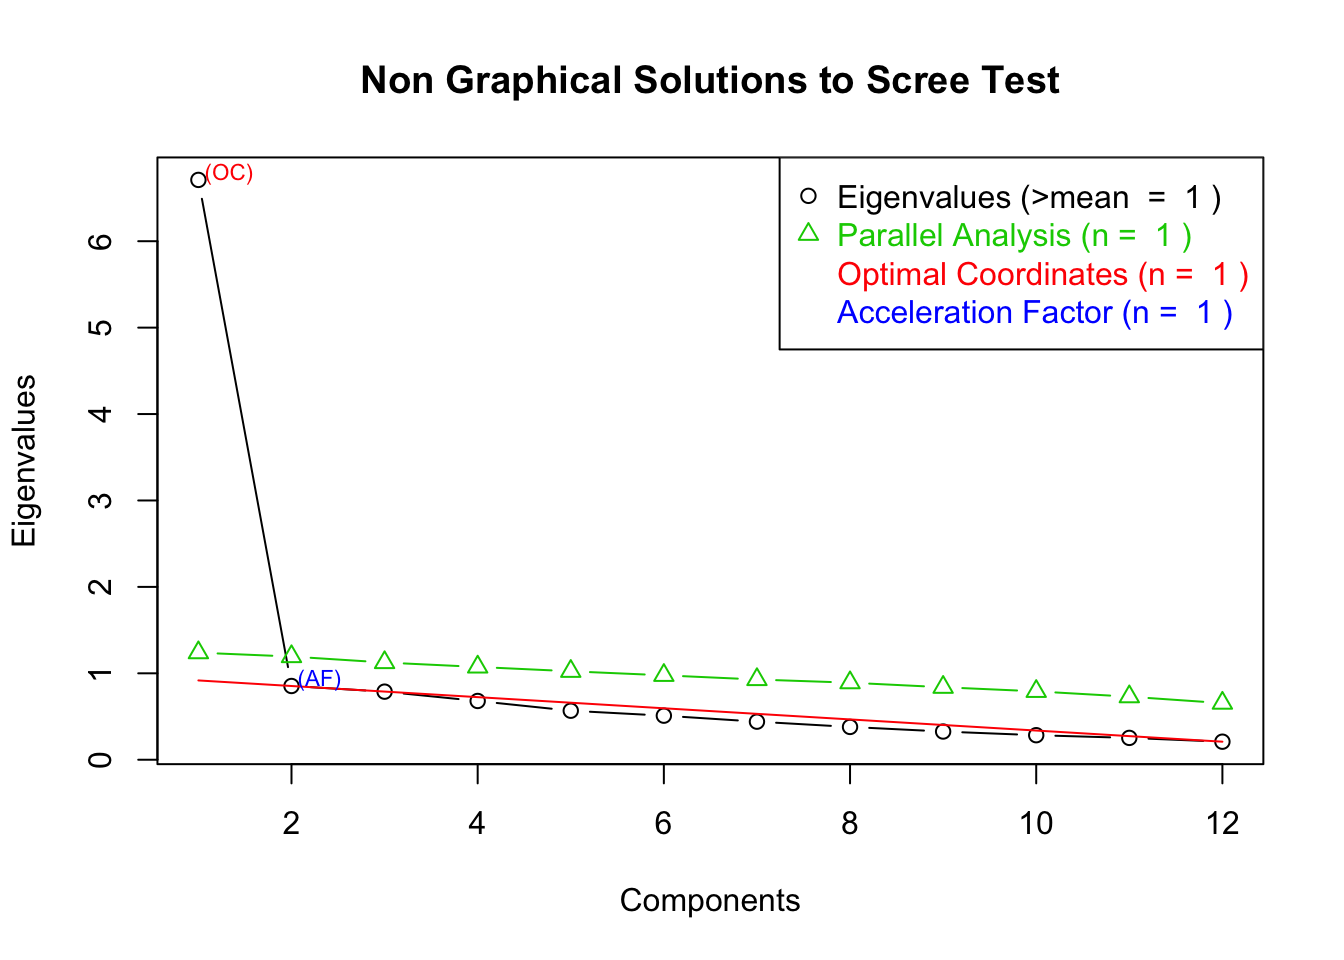
\includegraphics{tetc-analysis-submit_files/figure-latex/unnamed-chunk-6-1.pdf}

\begin{Shaded}
\begin{Highlighting}[]
\KeywordTok{ggsave}\NormalTok{(}\StringTok{"combined-plot.png"}\NormalTok{, }\DataTypeTok{width =} \DecValTok{12}\NormalTok{, }\DataTypeTok{height =} \DecValTok{7}\NormalTok{)}
\end{Highlighting}
\end{Shaded}


\end{document}
